\documentclass[preview]{standalone}

\usepackage[english]{babel}
\usepackage{amsmath}
\usepackage{amssymb}

\usepackage[]{tikz}
\begin{document}

\begin{center}
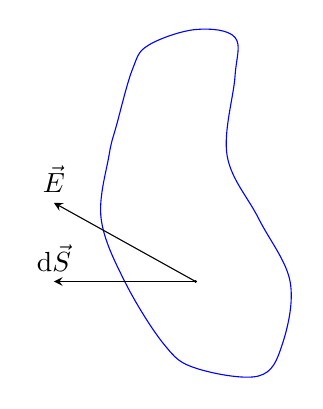
\begin{tikzpicture}[scale=2 ,>=stealth]
                      \begin{scope}[rotate=90]
                        \draw[blue] plot [smooth cycle, tension=0.6] coordinates {(4.4,0.4)(4.6,0.25)(5,0.2)(5.4,0.4)(5.8,0.6)(6.3,0.55)(6.55,0.55)(6.6,0.8)(6.5,1.1)(6.35,1.2)(6,1.3)(5.8,1.35)(5.4,1.4)(5,1.25)(4.6,1)(4.45,0.8)};
                        \draw[->] (5,0.8)--(5.5,1.7) node[above]{$\vec{E}$};
                        \draw[->] (5,0.8)--(5,1.7) node[above]{$\mathrm{d} \vec{S}$};
                        \filldraw[black] (5,0.8)circle(0.005);
                      \end{scope}
                    \end{tikzpicture}
\end{center}

\end{document}
